\chapter{Lecture \thechapter{} of 24/03/2026}

\begin{proposition}[Nonemptyness of relative interiors]

    Let $C \seq \R^d$ be convex and nonempty. Then: 

    \begin{enumerate}
        \item[a)] the set $\ri{C}$ is a nonempty convex set, $\aff{\ri{C}} = \aff{C}$;
        \item[b)] if $m = \mathrm{dim}_\R \left(\aff{C}\right), \, m>0$ then there exists $m+1$ vectors $x_0,x_1,\dots,x_m \in \ri{C}$ such that 
            \[ \aff{C} = \mathrm{span}\set{x_1 - x_0, x_2 - x_0, \dots, x_m - x_{0}}. \]
    \end{enumerate}
    
\end{proposition}

\begin{proof}
    
    The fact that $\ri{C}$ is convex is a consequence of LSP. We have to show that $\ri{C}$ is nonempty. Without loss of generality, we can assume $0 \in C$ (up to a traslation), consider $\aff{C}$. If $m = 0$ then $C = \set{0} \implies \ri{C} = C$ as for any $r > 0$, $B(0,r) \cap \aff{C} = C$. Assume now $m > 0$. Consider $z_1,\dots,z_m \in C$ linearly independent such that $\aff{C} = \mathrm{span}\set{z_1,\dots,z_m}$. Considet the set 

    \[ X = \set{x : x = \sum_{i=1}^m \alpha_i z_i,\,\alpha_i > 0,\, \sum_i \alpha_i < 1}. \]

    The strategy now is to prove that $X \seq \ri{C}$. Observe that $X \seq C$. Fix $\bar{x} \in X$, $x \in \aff{C}$ and observe that 
    
    \begin{align*}
        \bar{x} &= Z \bar{\alpha},\, \bar{\alpha } \in \R^m \\
        x &= Z \alpha \, \alpha \in \R^m
    \end{align*}

    with $Z$ the matrix with coloumns $z_1,\dots,z_m$. Notice that 

    \begin{align*}
        \norm{x - \bar{x}}^2 &= \langle Z(\alpha - \bar{\alpha}), Z(\alpha - \bar{\alpha}) \rangle \\
            &= (\alpha - \bar{\alpha})^\top Z^\top Z (\alpha - \bar{\alpha}) \\
            &\le \gamma \norm{\alpha - \bar{\alpha}}^2.
    \end{align*}

    Since $\bar{x} \in X$, the vecotr $\bar{\alpha} \in A = \set{\alpha \in \R^m : \sum_{i} \alpha_i < 1, \, \alpha_i > 0}$ which is an open set. If $x$ is suficently close to $\bar{x}$, then $\alpha$ is clost to $\bar{\alpha}$ by the above estimate on the norm. This implies that $\alpha \in A$, hence $x \in X$, so $B(\bar{x},r) \cap \aff{C} \seq X \seq C$. This shows that $X \seq \ri{C}$.

    Notice that, by construction, $\aff{X} = \aff{C}$, hence $\aff{X} \seq \aff{\ri{C}} \seq \aff{C}$.

    \paragraph{b):} fix $x_0 \in \ri{C}$ ($x_0$ exists by a)), translate $C$ to $C - x_0$, so that $0 \in C - x_0$. fix $z_1,\dots,z_m \in C - x_0$ linearly independent such that $\aff{C - x_0} = \mathrm{span}\set{z_1,\dots,z_m}$. Let $\alpha \in (0,1)$ and consider $(1-\alpha)\cdot 0 + \alpha z_i \in \ri{C-x_0}$ by LSP as $0,z_i \in \ri{C-x_0}$. Hence $\alpha z_i \in \ri{C-x_0}$. It follows that the vectos $x_i = x_0 + \alpha z_i$ are such that $x_1 - x_0, \dots, x_m-x_0$ spans the parallel space.

\end{proof}

\begin{lemma}[Prolungation lemma, Book 1.3.3]

    Let $C \seq \R^d$ convex nonempty. A vector $x \in C$ belongs to $\ri{C}$ if and only if for any $\bar{x} \in C$ there exists a $\gamma > 0$ such that $x + \gamma(x - \bar{x}) \in C (*)$, i.e. every line segment connecting $x$ to any $\bar{x}$ can be prolongated beyond $x$ without leaving $C$.
    
\end{lemma}

\begin{proof}
    
    ''$\implies$'' easy. 

    Let $x$ satisfy $(*)$, fix $\bar{x} \in \ri{C}$ (it exists thanks to the above proposition). If $x = \bar{x}$ then $x \in \ri{C}$ and we are happy. If not, there exists a $\gamma > 0$ such that $z = x + \gamma(x-\bar{x}) \in C$ so that $x$ lies within the line segment connecting $\bar{x}$ and $z$. By LSP, it follows that $x \in \ri{C}$.

\end{proof}

\begin{proposition}[Minima of concave funcitons]
    
    Let $X \seq \Rn$ be convex and nonempty. Let $f : X \to \R$ be concave. Define 

    \[ X^* = \arg\min_{x \in X} f(x). \]

    If $X^* \cap \ri{X} \neq \emptyset$, then $f$ is constant.

\end{proposition}

\begin{proof}
    
    Assume $x^* \in X^* \cap \ri{X}$, by prolongation lemma, there exists $\gamma > 0$ such that the point $\hat{x} = x^* +\gamma(x^* - x)$ belongs to $X$, implying that

    \[ x^* = \frac{1}{\gamma + 1}\hat{x} + \frac{\gamma}{\gamma + 1}x. \]

    By concavity of $f$, 

    \begin{align*}
        f(x^*) &= f(\frac{1}{\gamma + 1}\hat{x} + \frac{\gamma}{\gamma + 1}x) \\ 
            &\ge \frac{1}{\gamma+1} f(\hat{x}) + \frac{\gamma}{\gamma+1}f(x). 
    \end{align*}

    Since $x^*$ is a minimum point, it must be that $f(y) \ge f(x^*)$ for any $y$, in particular, $f(\hat{x}) \ge f(x^*)$ and $f(x) \ge f(x^*)$, hence $f(x) = f(x^*)$ for any $x$.

\end{proof}

An immediate consequence is that if $f(x) = a^\top x$ with $a \in \Rn$, then the minima of this function is attained at the boundary of its domain (which is assumed to be convex).

\begin{proposition}[Continuity of convex funcitons, Book 1.3.11]
    
    If $f : \Rn \to \R$ is convex, then $f$ is continous. More generally, if $f : \Rn \to \Rb$ is proper and convex, then the restriction of $f$ to $\dom{f}$ is continous in $\ri{\dom{f}}$.

\end{proposition}

\begin{proof}
    
    Assume $0 \in \dom{f}$ (if not translate). Without loss of generality, assume that the set $X = \set{x : \norm{x}_\infty \le 1} \seq \dom{f}$ (up to dilatation). It is now sufficent to prove that $f$ is continous at $0$: for any sequence $\set{x_k}_k$ such that $x_k \to 0$ we want to prove $f(x_k) \to f(0)$. Define $e_i$, for $i = 1,\dots,2^n$ the corners of $X$. Let $x \in X$, then 

    \[ x = \sum_{i=1}^{2^n} \alpha_i e_i\quad \sum_i \alpha_i = 1, \, \alpha_i \ge 0. \]

    Then 

    \begin{align*}
        f(x) &= f\left(\sum_{i=1}^{2^n} \alpha_i e_i\right) \\
            &\le \sum_i \alpha_i f(e_i) \\
            &\le \sum_i \alpha_i \left(\max_j f(e_j)\right) \\
            &\le \max_j f(e_j).
    \end{align*}

    Consider now the sequence $x_k \to 0$, define $y_k = x_k/\norm{x_k}$, $z_k = -x_k/\norm{x_k}$. We can see $x_k$ as a convex combination of $y_k$ and 0, hence 

    \begin{align*}
        f(x_k) &= f(\norm{x_k}_\infty y_k - (1-\norm{x_k}_\infty)\cdot 0) \\ 
            &\le \norm{x_k}f(y_k) + (1-\norm{x_k})f(0).
    \end{align*}

    Observe that $\norm{x_k} \to 0$, and $f(y_k)$ is bounded ($y_k \in \dom{f}$), hence $\norm{x_k}f(y_k) \to 0$ as $k \to +\infty$. This shows that 

    \[ \limsup_k f(x_k) \le f(0). \]

    DFor $z_k$ instead:

    \begin{align*}
        f(0) &= f\left(\frac{1}{1+\norm{x_k}}x_k + \frac{\norm{x_k}}{1+\norm{x_k}}z_k\right) \le \liminf_k f(x_k).
    \end{align*}

    Hence $f(0) \le \liminf_k f(x_k) \le \limsup_k f(x_k) \le f(0)$. This shows that $f$ is continous at 0.

\end{proof}

\section{Intermezzo}

Let $E \seq \Rnp$, $f : D \to \Rb$ where $D = \set{x \in \Rn : \exists\, w \in \R \text{ s.t } (x,w) \in E}$, $f(x) = \inf_w (x,w) \in E$.

Let now $f : X \to \Rb$ any function. We define the \emph{closure of} $f$ as 

\[ \cl{f}(x) = \inf \set{w : (x,w) \in \cl{\epi{f}}}. \]

The \emph{convex closure} of $f$ is 

\[ \ccl{f}(x) = \inf\set{w : (x,w) \in \cl{\conv{\epi{f}}}}. \]

It can be proven that $\ccl{f} = \cl{F}$ where 

\[ F(x) = \inf\set{w : (x,w) \in \conv{\epi{f}}}. \]

\begin{figure}[ht!]
    \centering
    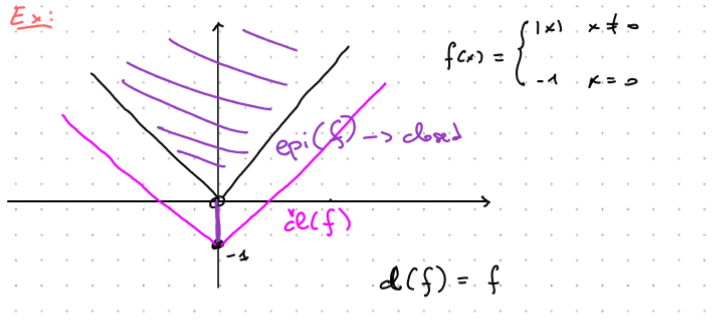
\includegraphics[width=0.7\textwidth]{img/convcl.png}
    \caption{Example of convex closure of a function}
\end{figure}

\begin{proposition}[Book 1.3.13]
    
    Let $f : X \to \Rb$. Then 

    \[ \inf_{x \in X} f(x) = \inf_{x \in \Rn} \cl{f}(x) = \inf_{x \in \Rn} F(x) = \inf_{x \in \Rn} \ccl{f}(x). \]

\end{proposition}

\begin{proof}
    
    If $\epi{f} = \emptyset$, then $f \cong +\infty$, so this case is verified. Suppose now $\epi{f} \neq \emptyset$. Let $f^* = \inf_{x \in \Rn} \cl{f}(x)$. for any sequence $\set{(\bar{x}_k, \bar{w}_k)}_k \seq \cl{\epi{f}}$ with $\bar{w}_k \to f^*$ we can construct a subsequence $\set{(x_k, w_k)}_k \seq \epi{f}$ such that $w_k \to f^*$, $\abs{w_k - \bar{w}_k} \to 0$. For each $x_k \in X$, it holds $(x_k,w_k) \in \epi{f}$, then $f(x_k) \le w_k$. But then 
    
    \[ \inf_{x \in X} f(x) \le \limsup_k f(x_k) \le \lim_k w_k = f^* \le \cl{f}(x) \le f(x). \]

    Hence 

    \[ \inf_{x \in X} f(x) = \inf_{x \in \Rn} \cl{f}(x). \]

    The next part uses the same argument.

\end{proof}


